% Notes on Iron lines:
%171 = Fe IX 5.9
%195 = Fe XII 6.2 
%284 = Fe XV 6.3
%335 = Fe XVI 6.3

\section{Introduction}\label{sec:intro}
	
	An essential tool used to study remote solar phenomena is the spectrograph.
	By more closely examining the wavelength of light emitted from the sun we gain access to a wealth of information (temperature, density, velocity, etc.) needed to more completely describe the solar plasma and properly inform our models.
	Slit spectrographs take a very narrow strip of the sun and disperse the light emitted using a diffraction grating, providing high spectral resolution over a very small spatial field of view.
	Spectrally resolved images are then built by rastering the slit over a region of interest, requiring a full exposure at every position, which can take on the order of hours to cover a large portion of the solar disk.
	
	An alternative approach is to remove the slit, a \emph{slitless} spectrograph.
	Slittless spectrographs disperse an image over a larger field of view.
	The data from these instruments, sometimes called overlapograms, have spatial and spectral information overlapped in the dispersive direction.
	Slitless spectrographs often image in multiple spectral orders, each with a different blend of spatial and spectral information, that can be combined and ``inverted'' to form a spectrally resolved image of the sun at every exposure.
	By doing so these instruments trade spatial and spectral resolution for much higher cadence.
    
	Slitless spectrographs have been used infrequently for decades to image the sun and have recently regained popularity.
	Only two satellite missions have routinely captured solar slitless spectrograph data: The S082A instrument on {\it Skylab} \citep{Tousey1973} and the Res-K instrument of the Russian KRONOS-I mission \citep{Zhitnik1998}.
	These two instruments have informed the recent development and proposal of another 
	full disk slitless spectrograph, the COronal Spectroscopic Imager in the EUV  \citep[COSIE:][]{winebarger2019,golub2020}.
	The currently operating Extreme-ultraviolet Imaging Spectrograph \citep[EIS:][]{culhane2007}) on the {\it Hinode} mission \citep{kosugi2007} includes 40$^{\prime\prime}$ and 266$^{\prime\prime}$ slots that can produce overlappogram that has been used in a limited number of quantitative studies \citep{harra2017,harra2020}.
	In addition to these satellite missions several sounding rocket based slitless spectrographs have recently imaged the sun including The Multi-Order Solar Extreme ultraviolet Spectrograph \citep[MOSES:][]{Fox2011}, the Extreme ultraviolet Snapshot Imaging Spectrograph \citep[ESIS:][]{ESIS,Parker2021}, and the recently launched Marshall Grating Incident X-ray Spectrometer \citep[MaGIXS:][]{MaGIXS} that was flown with a $12' \times 33'$ slot.
	
	MOSES was launched for the first time from White Sands Missile Range on February 8th, 2006.
	The primary science goal of MOSES was to measure line profiles in \heii \ over a wide field of view ($\approx 20' \times 10'$) at every exposure.
	By imaging in multiple orders simultaneously, $m = -1, 0, \text{\ and\ } 1$, MOSES captures three different projections through a spatial-spectral cube, $I(x,y,\lambda)$, that can be combined and inverted to return a line profile at every pixel over its large field of view, at every exposure.
	Various inversion methods have been used to return line profiles thus far, mostly for small explosive events in \heii\ \citep{Fox2010,Fox2011,Courrier2018,Rust2019}.
	
	Early work with MOSES images revealed faint solar features when subtracting different spectral orders, as well as in the residuals while inverting, that could not be attributed to \heii.
	These features could not be attributed to the most obvious sources of spectral contamination, including the nearby \sixi, or two bright Iron lines, \fexv\ and \fexvi.
	The periodic multi-layer coatings used on the MOSES primary and secondary optics were designed to allow for optimal throughput at 304\,\AA \ but to suppress the close Iron lines, \fexv\ and \fexvi, as much as possible \citep{Owens2005} making them an unlikely source of contamination.
	Moreover, if much of the contamination were attributable to one of these strong lines, then the contaminant features should appear twice in the difference images: once at the correct location on the Sun, and then in inverted intensity at a predictable offset; yet such a pattern was not observed \citep{Fox2011}.
	\sixi, which is too close in wavelength to be removed by the MOSES multi-layer coating was always expected to be a contamination source in the data.
	With a spectral dispersion of \spectdisperspix\ (\spectdispersvel), features in \sixi \ are dispersed roughly \sixipix\ pixels from \heii \ and therefore are easily distinguishable features in \heii.
	Therefore these unexpected solar features must be from emission at dimmer and less obvious wavelengths in the MOSES passband.
	In this paper we identify and quantify the sources of spectral contamination in the MOSES images.
	We also comment on the MOSES design decisions that led to this confusion, and how similar instruments can be adapted to better control spectral contamination.
	
	In Section \ref{sec:data} we present a time averaged set of images from the 2006 MOSES flight, as well as 4 co-temporal and co-aligned images from SOHO EIT.
	We also discuss the unexpected solar features of unknown spectral content found in the MOSES data.
	Section \ref{sec:methods} describes our methods for identifying and quantifying sources of spectral contamination.  
	This includes using the cross-correlation of MOSES difference images as an indication of significant spectral contamination (Section \ref{sec:crosscorrelation} and \ref{sec:sigtesting}) and how we combine data from EIT with synthetic spectra from the Chianti database \citep{ChiantiI,ChiantiX} to generate synthetic MOSES images that can be fit to MOSES images (Section \ref{sec:fomod}).
	Section \ref{sec:results} shows our best fit to the MOSES data, the resulting spectral content of the time averaged MOSES images.
	We discuss our results and their implications for future missions of this kind in Section \ref{sec:conclusion}.   


\section{Data}\label{sec:data}

%	Sticking this here for now:
%	
%	The MOSES wavelength passband is defined by its diffraction grating and periodic multi-layer mirror coatings.
%	The primary grating of MOSES causes some wavelength selection in the outboard orders, but none in the central order.
%	Even in the outboard orders, the MOSES grating alone, with a spectral dispersion of \spectdisperspix, is insufficient to isolate \heii \ from its near neighbors, the brightest being \sixi, \fexv, and \fexvi.
%	To further isolate \heii\ in the outboard orders, and define a passband for the zeroth order, MOSES uses a narrowband metallic multi-layer coating on both the primary grating and secondary fold flat optics.
%	
%	Metallic multi-layer coatings are almost ubiquitous in normal incidence solar EUV telescopes \citep{Windt2015}, the most notable current example being the Atmospheric Imaging Assembly \citep[AIA:][]{lemen2011} onboard the Solar Dynamics Observatory (SDO).
%	Periodic multi-layers provide excellent reflectivity and narrow enough passbands for imaging isolated and bright EUV spectral lines.
%	Despite their high performance, current technology only allows periodic multi-layers to be so narrow, allowing non-negligible contributions from other lines in the instrument passband \citep{AIA-Response}.
%	
%	The MOSES multi-layer coatings were designed to allow for optimal throughput at 304\,\AA \ but to suppress the close Iron lines, \fexv\ and \fexvi, as much as possible \citep{Owens2005}.
%	The next closest bright line to \heii\ is \sixi, which is too close in wavelength to be removed by the MOSES multi-layer coating.
%	\sixi\ was always expected to be a contamination source in the data.
%	With a spectral dispersion of \spectdisperspix\ (\spectdispersvel), features in \sixi \ are dispersed roughly \sixipix\ pixels from \heii \ and therefore are easily distinguishable from even the fastest events in \heii.

	\subsection{MOSES}\label{sec:MOSES_data}
	
		The MOSES sounding rocket launched from White Sands Missile Range on February 8th, 2006 at 18:44 UT. 
		It recorded 27 exposures between 18:44:17 and 18:49:13 UT above $\sim 160$\, km in altitude, an altitude which roughly corresponds to 50\% atmospheric transmission for 304\,\AA\ radiation.  
		Exposure times ranged from .25 - 24 seconds with a roughly 6 second readout time in between.  
		An exposure consists of three images, one for each of the three spectral orders $m = -1, 0, \text{\ and\ } 1$.
		For the rest of the paper we will refer to the $m$th order MOSES image as, $I_m$.  
		All data was dark subtracted and co-aligned to exposure number 13 prior to our study \citep{Fox2010}. 
		
    	To increase signal to noise, we form a single time averaged image in each spectral order. The wide range of exposure times obtained during the flight guarantees that well exposed, unsaturated intensities are available at every spatial location.
    	Saturated pixels are replaced with IEEE NaN (Not a Number) and treated as missing data.
		Since MOSES observes through a time-varying column of atmosphere throughout its flight, we use the median of each image as a proxy for exposure time, rather than the amount of time the shutter is open.
		At each spatial pixel, in each spectral order, the average intensity is the sum over time of unsaturated intensities divided by the sum of their proxy exposure times. This procedure also renormalizes the three MOSES spectral orders to the same sensitivity.
		The top row of Figure \ref{fig:moses_super} shows the time averaged versions of $I_1$ and $I_0$. 
		
		
		\begin{figure}
			\centering
			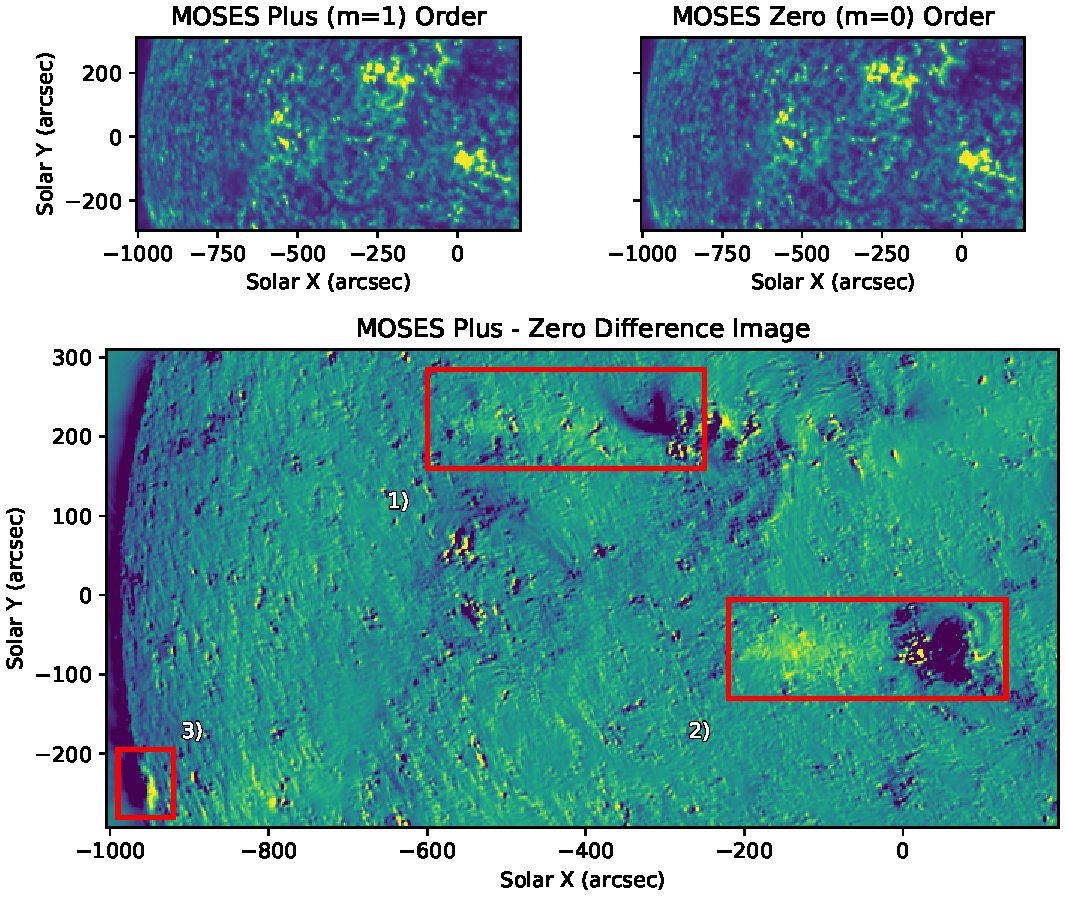
\includegraphics[width=\linewidth]{moses_dif}
			\caption{Time averaged images for the m = 0 and 1 spectral orders (top row), followed by their difference, m = 1 minus m = 0.  Regions one through three, boxed in red, show regions of high spectral contamination. Dark features from the m = 0 order are adjacent to white smears with pixel shifts too large to be Doppler shifts.}
			\label{fig:moses_super}
		\end{figure}
	
		
		Identifying solar features in the MOSES data that originate at wavelengths different from \heii\ is simple. 
		Subtracting $I_0$ (that contains no spectral dispersion) from either outboard order ($I_{+1}$ or $I_{-1}$) eliminates 303.8\,\AA\ features. 
		What remains are bipolar features of various spatial scales along the dispersion direction, which is horizontal.  
		A feature in the principle spectral line, \heii, with a nonzero line-of-sight (LOS) velocity is translated along image rows.    
		MOSES has a spectral dispersion of \spectdispersvel, leading to a less than ten pixel shift for even the fastest LOS velocities in He\,{\sc ii}. 
		This results in a bipolar feature with an obvious positive and negative counterpart that are immediately next to one another. Events like these have been studied in detail by several authors \citep{Fox2011,Courrier2018,Rust2019}.
		
		Features from other emission lines in the MOSES passband have shifts larger than 10 pixels and cannot be mistaken as Doppler shifted features in \heii. 
		A feature in \sixi, the next closest line, would be shifted by \sixipix\ pixels. 
		Si\,{\sc xi} features can be seen just above the solar limb, where He\,\textsc{ii}\ has little to no contribution. 
		The best example of this is region 3 boxed in red in Figure \ref{fig:moses_super}.  
		Box 1 of Figure \ref{fig:moses_super}c has a large, coherent, negative feature dubbed the ``wishbone''.  
		The wishbone is very solar in appearance and has no obvious positive counterpart.  
		Close inspection reveals a white smear to its left that is likely a shifted wishbone in the plus order.  
		Unfortunately the positive portion of the wishbone is too blurry to quantify its shift by inspection. 
		A previous study of these features by \citet{Rust2017} used a wavelet transform to isolate large scale features prior to taking the difference.  
		That procedure allowed \citet{Rust2017} to roughly identify a contribution from \spectralline{Mg}{viii}{315}\ to regions 1 and 2.
		\citet{Rust2017} also identified a faint copy of the limb, $\approx$200$^{\prime\prime}$ to the right of region 3 that was attributed to Si\,{\sc ix}/ Fe\,{\sc vi}\ 296.1\,\AA.
		Although the probable sources of contamination were identified, their contributions to the total image intensity were not quantified.
	
	\subsection{EIT}\label{sec:EIT_data}
		\begin{figure}
			\centering
			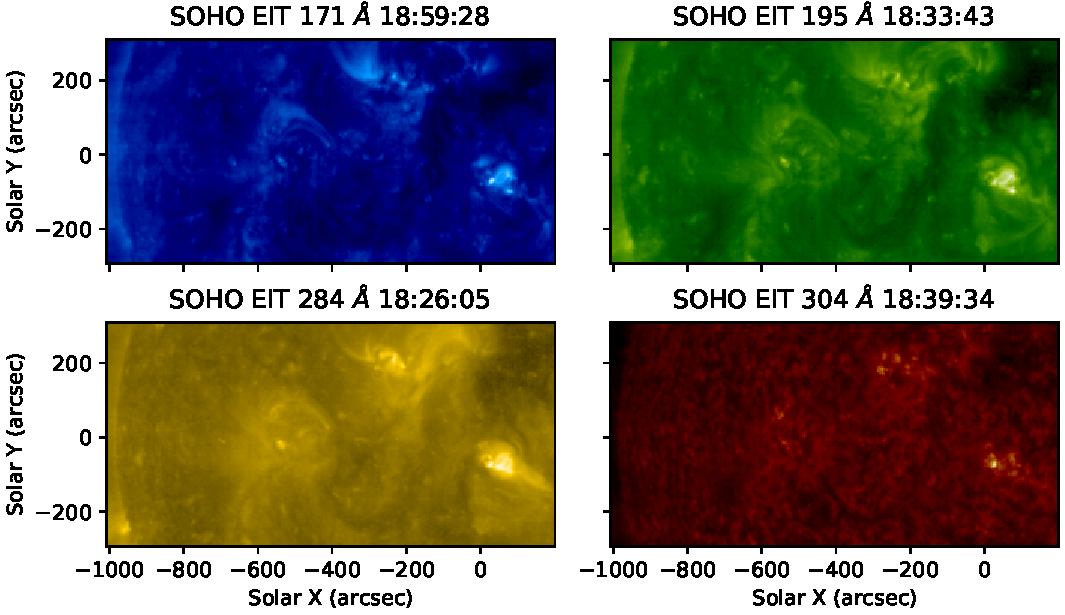
\includegraphics[width=\linewidth]{eit}
			\caption{SOHO EIT Images taken closest the MOSES Launch on February 8th, 2006. Each image was rotated to 2006-02-08 18:47 UT to match the middle MOSES exposure time.  After rotation, the EIT 304 channel was linearly co-aligned to the MOSES zero order, and then the same transformation was applied to every other channel.  Each image has been fourth root scaled.}
			\label{fig:EIT}
		\end{figure}
	
		The Extreme ultraviolet Imaging Telescope \citep[EIT:][]{EIT} on board the Solar and Heliospheric Observatory (SOHO) captured 4 full disk EUV images, one in each of the 171\,\AA, 195\,\AA, 284\,\AA, and 304\,\AA\ channels (Figure \ref{fig:EIT}) within $\approx20$ minutes of the 2008 MOSES flight.
		Prior to use, each image was first despiked using \texttt{iris\_prep\_despike.pro} with default settings and made level 1 with \texttt{eit\_prep.pro}. 
		They were then rotated to 2006-02-08 18:47 UT, the timestamp of image 13 of the MOSES observing sequence \citep{Fox2011}, using \texttt{drot\_map.pro}.
		EIT and MOSES were co-aligned by applying the affine coordinate transform to EIT 304\,\AA\ that maximized the zero-lag cross-correlation between it and the time averaged $m=0$ order image described in the proceeding subsection.
		The same transform was then applied to the other three EIT channels.
	 
		At first glance one can find several features in the MOSES difference image (Figure \ref{fig:moses_super}) that resemble features in the EIT 171, 195, and 284 images (Figure \ref{fig:EIT}).  
		The presence of these features in MOSES data indicates a contribution of coronal spectral lines to an otherwise transition region image.  
		While similarities between MOSES difference images and EIT images indicate the contribution of hotter lines to MOSES He\,{\sc ii} data, they do not straightforwardly tell how much, and by which lines.  
		In Section \ref{sec:methods} we set out to quantify the intensity contributed by each source of spectral contamination in the MOSES image.
		
		
\section{Methods}\label{sec:methods}
 	\subsection{Difference Image Cross-Correlation}\label{sec:crosscorrelation}
 	
 	 	\begin{figure}
 	 		\center
			\begin{tikzpicture}
			\newcommand{\toprow}{6.5}
			\newcommand{\columntwo}{8.5}
			
			%begin by adding a node for each figure
			\node[inner sep=0pt] (fig1) at (0,0)
			{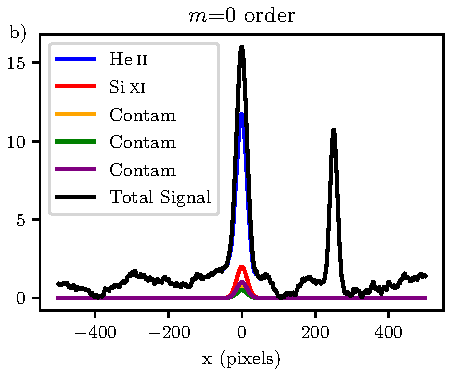
\includegraphics[]{fig1}};
			\node[inner sep=0pt] (fig2) at (0,\toprow)
			{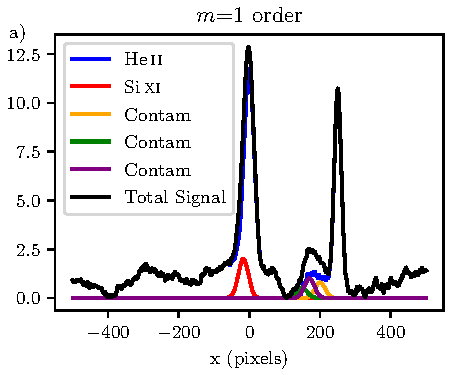
\includegraphics[]{fig2}};
			\node[inner sep=0pt] (fig3) at (0,-\toprow)
			{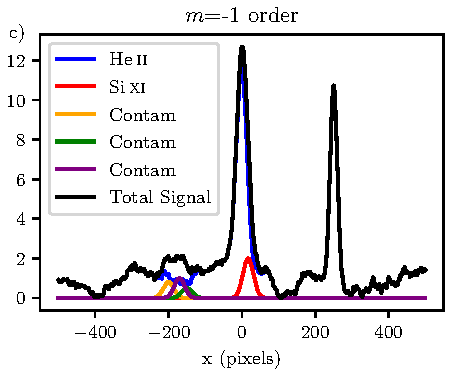
\includegraphics[]{fig3}};
			\node[inner sep=0pt] (fig4) at (\columntwo,\toprow/2)
			{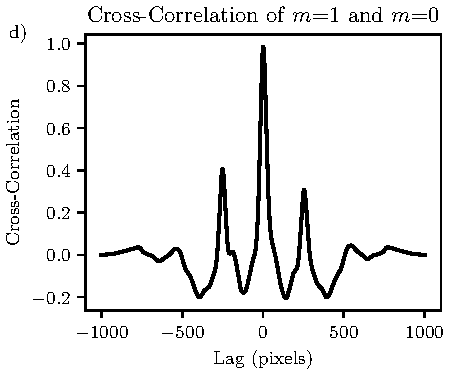
\includegraphics[]{fig4}};
			\node[inner sep=0pt] (fig5) at (\columntwo,-\toprow/2)
			{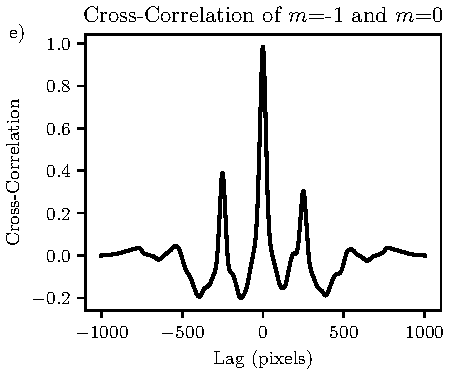
\includegraphics[]{fig5}};

			
			%add symbol for operation
			\node[inner sep=0pt](cc1) at (\columntwo/2,\toprow/2)
			{$\boldsymbol{\bigotimes}$};
			\node[inner sep=0pt](cc2) at (\columntwo/2,-\toprow/2)
{           $\boldsymbol{\bigotimes}$};

			
			%lets try drawing some lines between them.
			\draw[->] (fig1.east) -- (cc1.south);
			\draw[->] (fig2.east) -- (cc1.north);
			\draw[->] (cc1.east) -- (fig4.west);
			\draw[->] (fig1.east) -- (cc2.north);
			\draw[->] (fig3.east) -- (cc2.south);
			\draw[->] (cc2.east) -- (fig5.west);
			
			%draw a symbol legend
			\node(align)[draw] at (\columntwo,-\toprow/2-4) {
				\begin{tabular}{c}
				\tiny{$\bigotimes$ = Cross-Correlation}\\
				\end{tabular}};
			\end{tikzpicture}
 	 		\caption{Example 1D MOSES row in the $m$ = 1 (a), 0 (b), and -1 (c) spectral orders followed by the cross correlation of $m$=1 and 0 (d) and the cross-correlation of $m$ = -1 and 0 (e).  The cross-correlation of any two MOSES orders is dominated by the autocorrelation of stationary He\,{\sc ii} features and background making them less useful in identifying spectral content. The strong peaks in correlation at $\pm$250 pixels are the result of the two bright He\,\textsc{ii} features at 0 and 250 overlapping.}
 	 		\label{fig:methods1}
 	 	\end{figure}
 	 	
 	 	\begin{figure}
 	 		\center
 	 		\begin{tikzpicture}
 	 		\newcommand{\toprow}{6.5}
 	 		\newcommand{\columntwo}{8.5}
 	 		
 	 		%begin by adding a node for each figure
 	 		\node[inner sep=0pt] (fig1) at (0,0)
 	 		{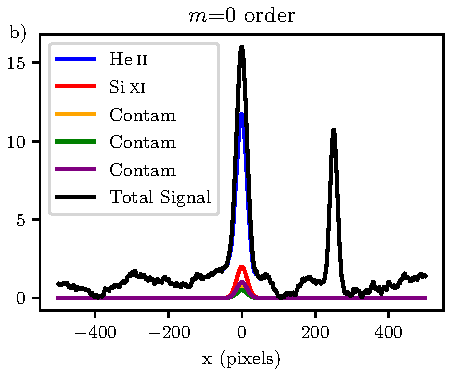
\includegraphics[]{fig1}};
 	 		\node[inner sep=0pt] (fig2) at (0,\toprow)
 	 		{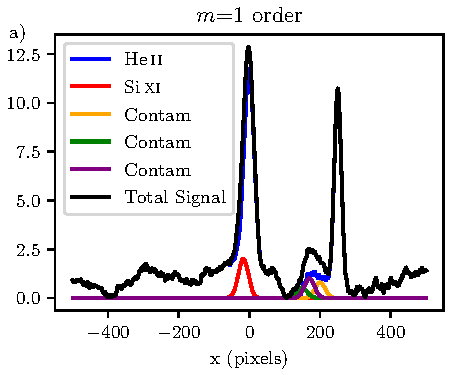
\includegraphics[]{fig2}};
 	 		\node[inner sep=0pt] (fig3) at (0,-\toprow)
 	 		{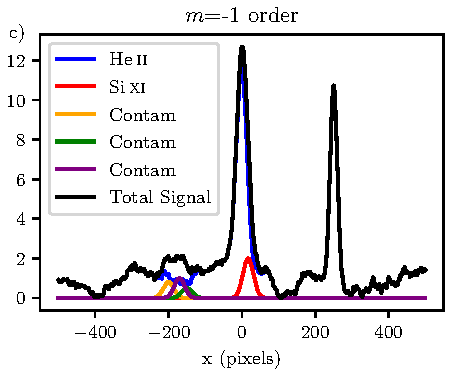
\includegraphics[]{fig3}};
 	 		\node[inner sep=0pt] (fig6) at (\columntwo,\toprow)
 	 		{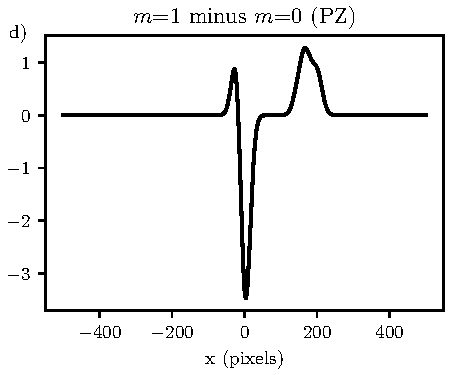
\includegraphics[]{fig6}};
 	 		\node[inner sep=0pt] (fig7) at (\columntwo,0)
 	 		{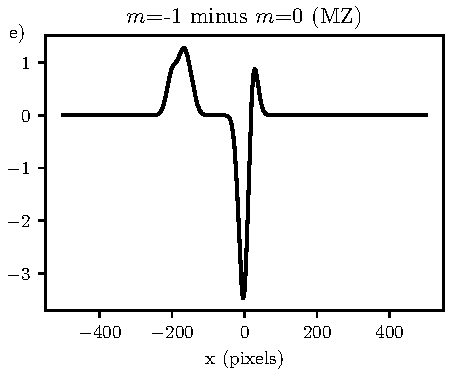
\includegraphics[]{fig7}};
 	 		\node[inner sep=0pt] (fig8) at (\columntwo,-\toprow)
 	 		{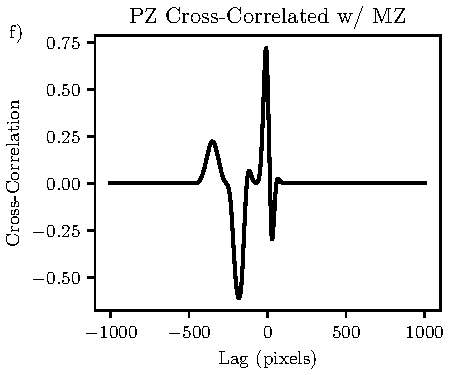
\includegraphics[]{fig8}};
 	 		
 	 		%add symbol for operation
 	 		\node[inner sep=0pt](dif1) at (4.25,+\toprow)
 	 		{$\boldsymbol{\bigtriangleup}$};
 	 		\node[inner sep=0pt](dif2) at (4.25,0)
 	 		{$\boldsymbol{\bigtriangleup}$};
 	 		\node[inner sep=0pt](cc1) at (\columntwo+4.2,0)
 	 		{$\bigotimes$};
 	 		\node[inner sep=0pt](t1) at (\columntwo+4.2,\toprow)
 	 		{};
 	 		\node[inner sep=0pt](t2) at (\columntwo+4.2,-\toprow)
 	 		{};
 	 		
 	 		
 	 		%lets try drawing some lines between them.
 	 		\draw[->] (fig1.north east) -- (dif1.south);
 	 		\draw[->] (fig2.east) -- (dif1.west);
 	 		\draw[->] (dif1.east) -- (fig6.west); 		
 	 		\draw[->] (fig1.east) -- (dif2.west);
 	 		\draw[->] (fig3.north east) -- (dif2.south);
 	 		\draw[->] (dif2.east) -- (fig7.west);
	
 	 		\draw[-] (fig6.east) -- (t1);
 	 		\draw[->] (t1) -- (cc1.north);
			\draw[->] (fig7.east) -- (cc1.west);
 	 		\draw[-] (cc1.south) -- (t2);
 	 		\draw[->] (t2) -- (fig8.east);

 	 		%draw a symbol legend
 	 		\node(align)[draw] at (4,-9.9) {
 	 			\begin{tabular}{l}
 	 			\tiny{$\bigotimes$ = Cross-Correlation} \\
 	 			\tiny{$\boldsymbol{\bigtriangleup}$ = Difference}
 	 			\end{tabular}};
 	 		
 	 		
 	 		\end{tikzpicture}
 	 		\caption{Example MOSES rows in $m = 1$ (a), 0 (b), and $-1$ (c) spectral orders.  Two difference images, $m=1$ minus $m=0$ (d) and $m=-1$ minus $m=0$ (e) are cross-correlated (e).  Taking a difference removes stationary He\,{\sc ii} features so that peaks in cross-correlation are indicative of extra spectral content.  Even in this simple example one cannot read off the spectral content of the MOSES images, demonstrating the need for a forward model.}
 	 		\label{fig:methods2}
 	 	\end{figure}
        
        To help identify signatures of hot spectral lines, we cross-correlated the MOSES difference images along the dispersion direction, or image rows.
        Performing a cross-correlation on the difference images requires justification.  
        An obvious first choice would have been to simply cross-correlate $I_0$ with either outboard order.  
        Unfortunately the correlation function is dominated by the autocorrelation of the He\,{\sc ii} signal as seen in Figure \ref{fig:methods1}d and \ref{fig:methods1}e.  
        These example cross-correlations show two main peaks in correlation that are due to the auto-correlation of bright He\,{\sc ii} features, and not spectral contamination.  
        This would also be the case when cross-correlating $I_{+1}$ and $I_{-1}$.  
        By taking the difference we remove stationary He\,{\sc ii} objects (Figure \ref{fig:methods2}d and \ref{fig:methods2}e) and, in turn, their autocorrelation from the cross-correlation function (Figure \ref{fig:methods2}f), leaving only peaks in correlation from features not of \heii.
 	
        The cross-correlation of two difference images along their rows is defined to be
        \begin{equation}
         \left(I_{+1}-I_0\right) \otimes \left(I_{-1}-I_0\right) = \mathcal{F}_x^{-1} \left\{\mathcal{F}_x\left(I_{+1}-I_0 \right)\mathcal{F}_x\left( I_{-1}-I_0)^* \right)  \right\},
         \label{eqn:cross_correlate}
        \end{equation}
        where $\mathcal{F}_x$ is the Fast Fourier Transform (FFT) operator applied along image rows.  
        % Prior to subtracting each image is normalized by its median \cck{(Didn't this renormalization already happen in \S\ref{sec:data}?)}.
        Also, image rows were padded with zeros, prior to applying the FFT to minimize effects of wrap-around. 
        Notice that edge effects are practically absent because of our choice to work with image differences. 
        Consequently, windowing was not necessary.
        This yields a one dimensional cross-correlation function for each row of the MOSES difference images.  
        Since we are concerned mostly with bulk spectral content we then take the mean of all 1024 cross-correlation functions, one for each row, to get our final correlation curve plotted in red in Figure \ref{fig:sigtest}. 
		 
		 \begin{figure}
		 	\centering
		 	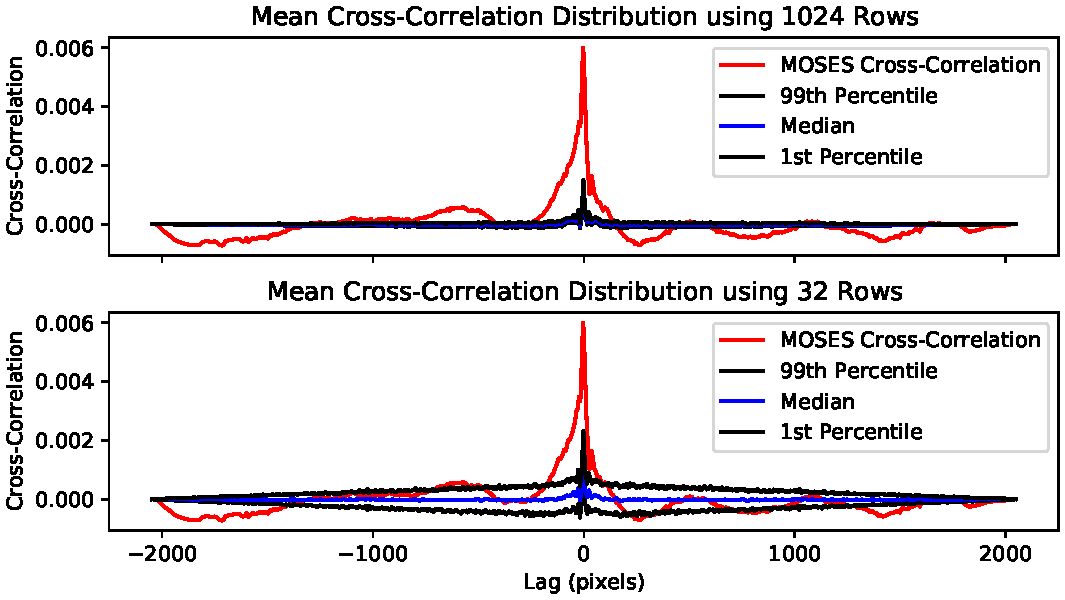
\includegraphics[width=\linewidth]{sigtest}
            \caption{The mean cross-correlation function of MOSES difference image rows (red) is compared to a distribution of mean cross-correlations from a selection of randomly generated test row differences (Section \ref{sec:sigtesting}). 
            The top panel shows the distribution after taking the mean of 1024 (the number of MOSES rows) randomly chosen test row differences 10,000 times.  
            The bottom panel challenges that all 1024 rows of MOSES are unique and shows the distribution for only 128 randomly chosen difference rows, also 10,000 times.  
            In either case the mean cross-correlation values from the MOSES data exceed the 98 percent confidence interval and are therefore deemed significant and indicative of spectral content in the MOSES data.}
		 	\label{fig:sigtest}
		 \end{figure}
		 
	 
		 The mean cross-correlation curve for the MOSES difference image has a few notable features.  
		 There are large%r 
		 peaks in correlation  at approximately $-1800$, $-500$, 250, 800, and 1500 pixel lags.  
		 The largest peak in correlation is centered about zero lag and is quite broad.   
		 While these features are identifiable, the curve is complicated enough that quantifying peaks in correlation visually is difficult and the significance of any given peak is questionable. 
		 We therefore move to test the null hypothesis that none of these features are the due to spectral contamination but are instead the result of random fluctuations in the data. 
		 We explore this null hypothesis in the next section by cross-correlating random data generated to emulate the scales present realistic solar features, such as those found in the MOSES image rows.
 
	
	\subsection{Significance Testing}\label{sec:sigtesting}
	
		The mean cross-correlation function of the two MOSES difference images, red in Figure \ref{fig:sigtest}, has several interesting peaks in correlation.  
		As can be seen in Figure \ref{fig:methods2}e, these peaks can be indicative of extra spectral content.  
		Actual MOSES images contain information not represented in the Figure \ref{fig:methods2} cartoon.  
		Each MOSES order has a slightly different point spread function and the He\,{\sc ii} features are not all stationary.  
		This leads to many extra small scale features in the difference images across the field of view.  
		It is also unclear what magnitude of cross-correlation we should expect from extra spectral content.  
		We therefore move to test the null hypothesis that the features in the MOSES difference image cross-correlation curve are the result of random correlations between each difference image and not indicative of extra spectral content.  
		
		
		To investigate the null hypothesis, we require test solar data that match the MOSES image rows in length and have similar power spectra and  autocorrelation.  
		MOSES images contain 2048 columns.  
		These columns have the same spatial features as MOSES image rows and the same noise distribution, but with none of the repeating patterns that arise from contaminant spectral lines.
		Therefore, MOSES images columns fairly represent how the MOSES image rows would appear under the null hypothesis.
		Despite this the MOSES image columns are insufficient for significance testing in two ways.  
		First, there is an insufficient sample size.
		With features in the MOSES images ranging from $\approx$ 4-100 pixels in size, we have at most 512 as few as 20 unique columns for significance testing.  
		Second, MOSES columns are half as long as the rows, preventing us from measuring the significance of correlation past 1024 pixel lag.  
		Therefore we require additional steps to generate a test data set for significance testing.
	
		Using the MOSES image columns as our basis we generated $N$ random arrays that are 2048 pixels long and resemble MOSES columns in structure.  
		First each time averaged MOSES image, $I_{mxy}$, is windowed with a Hanning window, $w_y$, and Fourier transformed along the column dimension, $y$.  
		The windowed Fourier transformed array is defined to be
	
		\begin{equation}
			\widetilde{I}_{mxk_y} = \mathcal{F}_y\left[ w_yI_{xy}\right]\quad.
			\label{eqn:ztwiddle}
		\end{equation}
% 		and the Hanning window is defined as \cck{I think there is no need to define the widely used Hanning window. As an aside: The awkward definition given in the IDL manual is generalized to include the Hamming window option as well, with $\alpha=0.54$. It is simpler to define the Hanning as $\frac{1}{2}(1-\cos).$}	
% 		\begin{equation}
% 			w_y = \alpha - (1-\alpha)\mathrm{cos}\left( \frac{2\pi y}{N} \right)\quad ,
% 			\label{eqn:Hanning}
% 		\end{equation}
% 		where $N$ is the number of elements in $y$ and $\alpha = .5$.
   		The spatial dimensions $x$ and $y$ represent MOSES image with $ x = 0,1,...,2047$ and $y = 0,1,...,1023$.
   	% 	\cck{\sout{Image columns were windowed prior to the Fourier transform so that the test data could be compared to the MOSES data with less influence from the discontinuity at the image edge.} (redundant with above)}  
	
		From the set of all the Fourier transformed data columns, we will generate a test \emph{row} for each order, $I'_{mx}$, by populating its Fourier transform, $\widetilde{I}'_{mk}$. 
		Each new array is formed by picking an element randomly from the distribution of Fourier transformed columns.
		Importantly, the same random choice is used to for each spectral order, $m$.
		The transformation outlined in Equation \ref{eqn:ztwiddle}
% 		and \ref{eqn:Hanning} 
		gives a distribution of 511 spatial frequency bins and one DC bin that each have 1024 elements (one from each column) for each order. 
		Once assembled, each array is further scrambled by giving each value of $k$, aside from the DC term, a random phase shift, $e^{i\phi}$, with $\phi \in (0, 2\pi]$ drawn from a uniform distribution. 
		The same random phase $\phi$ is employed for the $k^{\text{th}}$ Fourier component of each spectral order, producing three simulated rows that differ only according to the spectral order from which they were taken. 
		
		
% 		(see commented portion, which to me seemed unclear; I believe that the equation failed to capture the essential points.)
		
% 		By this method the $k^{\mathrm{th}}$ element in the $n^\text{th}$ test row, $\widetilde{I}'_{mkn}$, is
% 		\begin{equation}
% 			\widetilde{I}'_{mkn} = \widetilde{I}_{m\sigma k_y}e^{i\Phi} ,
% 			\label{eqn:synth_array}
% 		\end{equation}
% 		where $\sigma$ is a random integer between 0 and 2047 and $\Phi$ is a random phase between 0 and $2\pi$, both uniformly distributed and chosen $n$ times.
		
		%In order create an array that is 2048 elements long from one that is 1024 elements long we require twice as many values of $k$.
		%We solve this problem by double picking values from the distribution of $k_y$ for each wave number, $k$.  
		%The values of $k_y$ used in Equation \ref{eqn:synth_array} are,
		In order create an array that is 2048 elements long from one that is 1024 elements long we require twice as many values of $k$ as $k_y$:
		\begin{equation}\label{eq:freq_interp}
		    k_y = \begin{cases}
		        0,       & k=0,\\
		        \texttt{ceil}\left( \frac{k}{2} \right), & 0<k<1023,\\
		        511,        & k = 1023,\\
		        512,      & k = 1024,\\
		    \end{cases}
		\end{equation}
		%where $k = 1, 2,...,1022$ and \texttt{floor} rounds down to the nearest integer.
		where \texttt{ceil} rounds up to the nearest integer, and the $k$-indices are arranged as they traditionally are in the fast Fourier transform.
		Since our data is purely real we can fill in the remaining Fourier components,  negative frequencies, with the complex conjugate of the corresponding positive frequency component. 
		% The final $n^\text{th}$ test MOSES row
		Finally, all synthetic rows  of spectral order $m$ are found through an inverse FFT, 		
		\begin{equation}
			I'_{mxn} = \mathcal{F}_x^{-1}\left[\widetilde{I}'_{mkn}\right].
		\end{equation}
%		Again, this procedure is carried out for each order simultaneously.  
%		To best simulate a set of three MOSES rows, one for each order, when a frequency bin is assigned a value from the distribution, the same randomly generated indices are used for each order.  
%		For example, if the k$^{\mathrm{th}}$ frequency bin of a synthetic m = 0 order row, $I'_{0x}$, is selected to be $\widetilde{I}'_{0k} = \widetilde{I}\left[25, k  \right]e^{i\pi}$ from the 25$^{\mathrm{th}}$ element in the distribution with a $\pi$ phase shift, then the k$^{\mathrm{th}}$ element of the corresponding synthetic m = 1 and -1 rows is also  $\widetilde{P}_k^{'} = \widetilde{P}_w\left[25, k  \right]e^{i\pi}$ and  $\widetilde{M}_k^{'} = \widetilde{M}_w\left[25, k  \right]e^{i\pi}$.
        
%         \jdp{
% 		To verify that our 10,000 test arrays resemble the MOSES columns, we take a randomly selected 1024 element long section of each test \emph{row}, as well as the MOSES columns, and compare their power spectral and autocorrelation distributions. 
% 		We found fantastic agreement between the power spectral distribution of the real and test data.  
% 		In comparing their autocorrelations, we found the test data to have slightly higher autocorrelation in the tails of the distribution, or a wider distribution in general.
% 		This mismatch is a bit puzzling, considering the autocorrelation is simply the inverse Fourier transform of the power spectra.
% 		In the end a higher autocorrelation in the test data acts as a worse case scenario when comparing to the cross-correlation of MOSES rows and determining significance of peaks in correlation.
% 		}



We examined randomly drawn 1024-pixel segments from the 2048-pixel synthetic MOSES test rows and compared their power spectra to those of the original columns. 
The 10th percentile, median, and 90th percentile power spectra of both sets match extremely well, giving us confidence that our wavenumber interpolation scheme was properly implemented and yielded plausible distributions of intensity in the test rows.
		
% 		Figures \ref{fig:sigtestpower} and \ref{fig:sigtestauto}  show three percentiles of both power spectral and autocorrelation distributions (10th, 50th, and 90th) for $10,000$ test arrays. 
% 		Figure \ref{fig:sigtestpower} shows great agreement between test data and the MOSES columns in power spectral distribution.  
% 		Figure \ref{fig:sigtestauto} shows good agreement between the test data and MOSES columns at the median and only marginal agreement in the wings of the distribution.  
% 		Despite that the test rows most always has a higher autocorrelation length that the MOSES columns and therefore acts as a worse case scenario during significance testing.  
					
% 		\begin{figure}
% 			\centering
% 			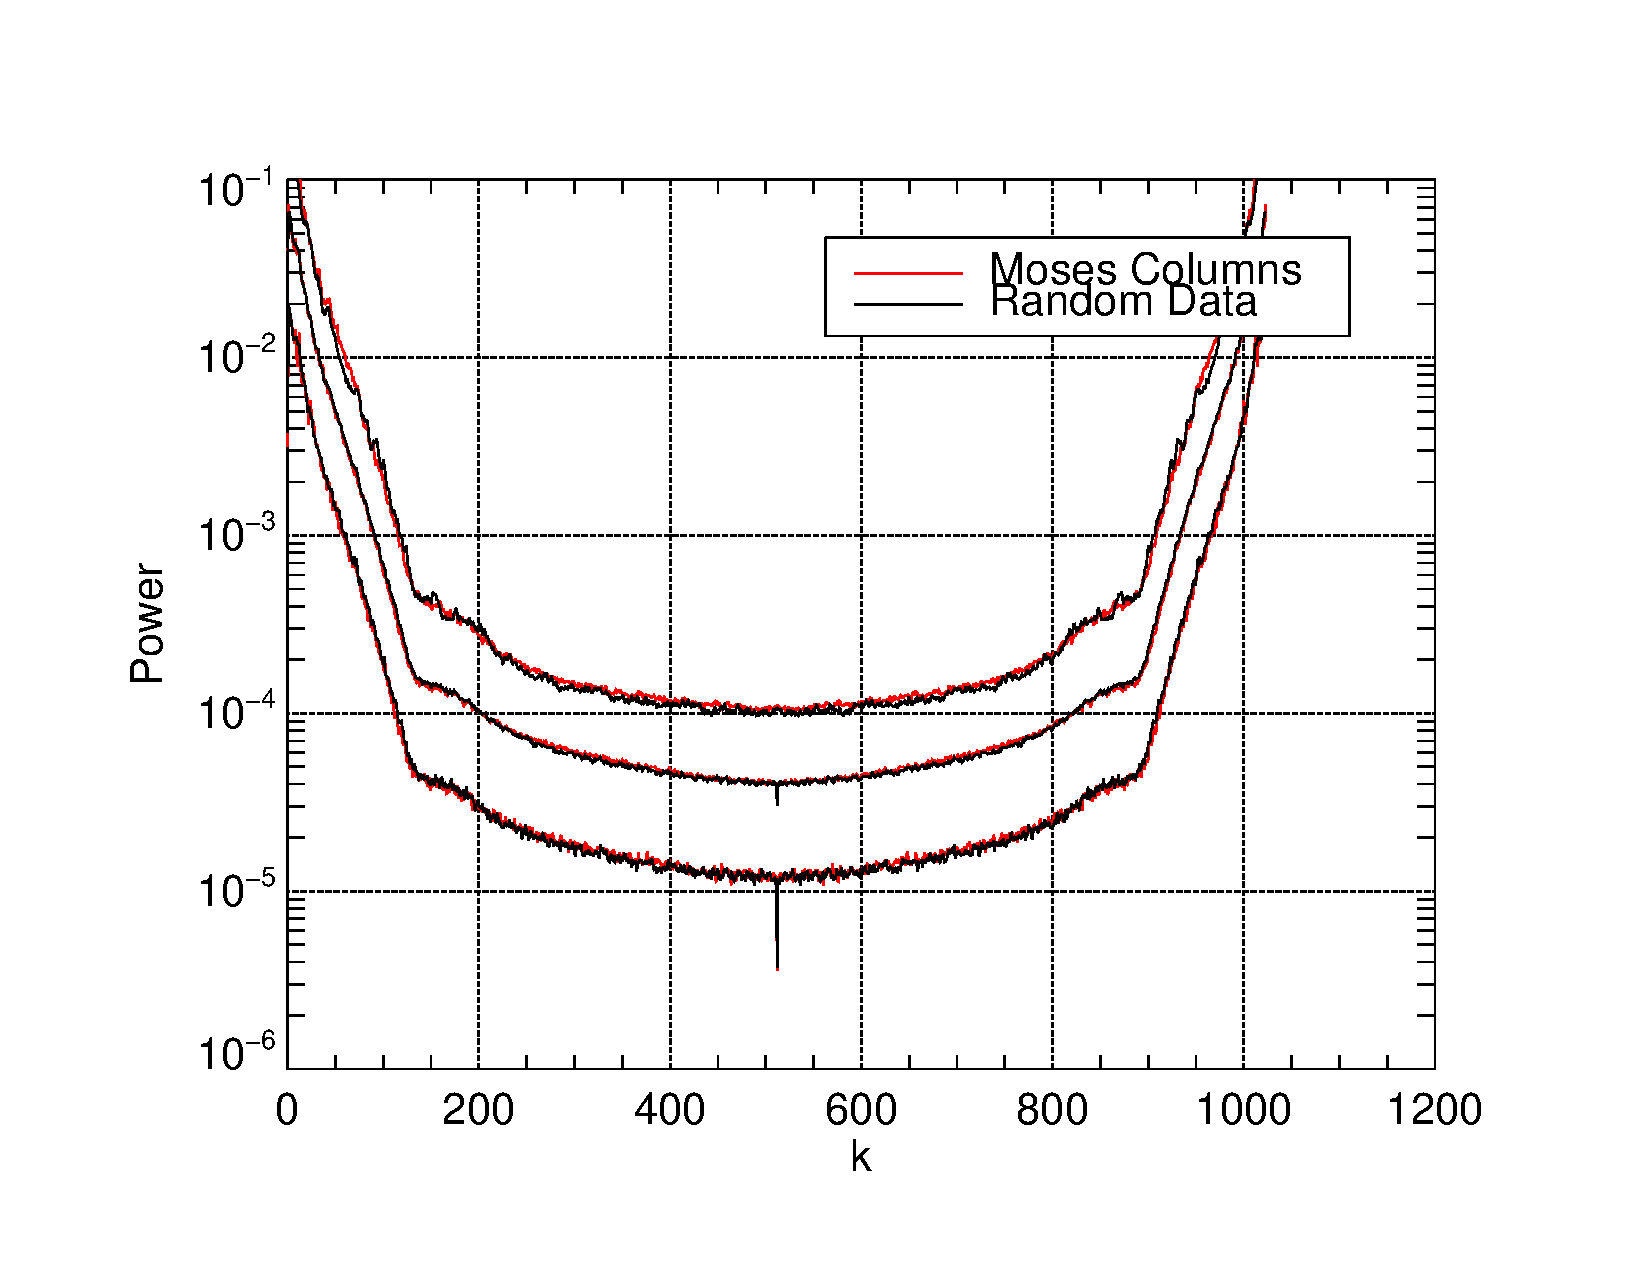
\includegraphics[width=\linewidth]{sigtestpower}
% 			\caption{The 10th, 50th, and 90th percentile of the power spectral distribution for each value of k is plotted for both the $m$ = 0 MOSES columns and test data.}
% 			\label{fig:sigtestpower}
% 		\end{figure}
% 		\begin{figure}
% 			\centering
% 			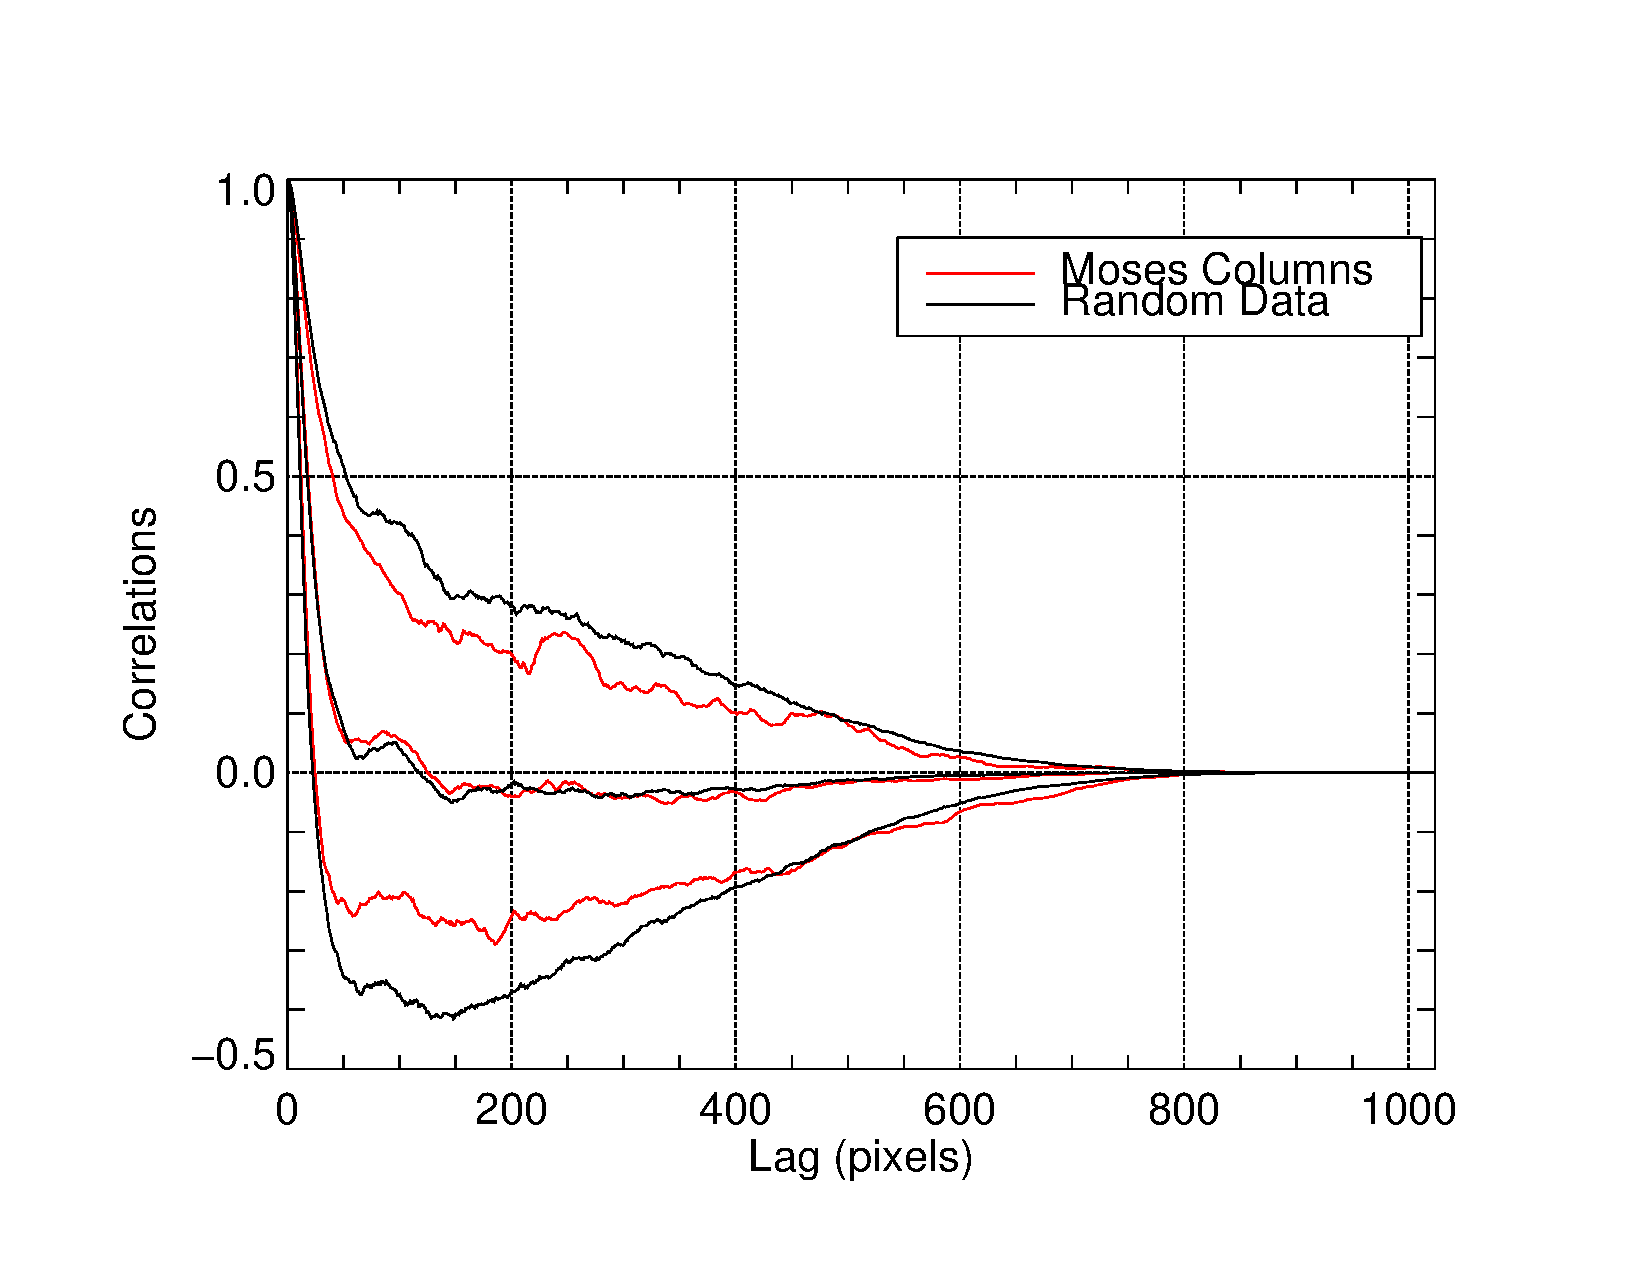
\includegraphics[width=\linewidth]{sigtestauto}
% 			\caption{The 10th, 50th, and 90th percentile of the auto-correlation distribution for each lag is plotted for both the $m$ = 0 MOSES columns and test data.}
% 			\label{fig:sigtestauto}
% 		\end{figure}
	
		Now that we have created a set of 10,000 test rows for each order $m$ we can cross-correlate the order-difference for each row, as we did for MOSES. 
% 		Every test row in each order, $I'_{mxn}$, is normalized by its median \cck{(Why? We hopefully began this synthesis exercise with columns extracted from median-normalized images. We do not do a row-by-row normalization of the MOSES data, correct?)}, and then subtracted and cross-correlated according to Equation \ref{eqn:cross_correlate}.
		This yields a set of $10,000$ test difference row cross-correlation functions.
		Since we are interested in the average MOSES difference row cross-correlation we choose a number of test row cross-correlations and average them together before comparison.
		The blue and black curves in the top panel of Figure \ref{fig:sigtest} shows the result of picking 1024 random test cross-correlations (the same number of rows as a MOSES image) and taking their average.
		We do this 10,000 times and form a distribution of mean cross-correlation values at each pixel lag.
		The $1^\text{st}$ and $99^\text{th}$ percentile of the distribution are plotted in black and the median in blue.
		From the top panel of Figure \ref{fig:sigtest} it is clear that a mean cross-correlation much greater or less than zero is highly unlikely in our test rows with no spectral content.
		The exception to this is at zero lag when a positive peak in correlation well above zero is typical.
		Despite this exception the peak in mean cross-correlation from the MOSES data is much greater, and broader, than that of the test data.
		The comparison in the top panel of Figure \ref{fig:sigtest} assumes that all 1024 difference rows from the MOSES data are unique.
		Since solar features in the MOSES images exceed a single pixel in size this is unlikely.
		The bottom panel of Figure \ref{fig:sigtest} is made in the same way as the top panel but uses the mean of only 32 rows when forming the distribution.
		We believe 32 independent rows represents a reasonable lower bound after examining the auto-correlation length of the MOSES rows and seeing a large fall off in autocorrelation ($\approx75$\% on average) by 32 pixel lag.
		Even when we assume that MOSES has only 32 unique rows we can see the same five large peaks in the MOSES mean cross-correlation (identified in Section \ref{sec:crosscorrelation}) fall outside the 98 percent two-sided confidence interval.
		
		
		From this study we find that the shape and magnitude of the largest peaks in the mean cross-correlation of the MOSES difference images are significant and indicative of spectral content.
		We therefore wish to quantify that spectral content.
		
			
	
	\subsection{Forward Model}\label{sec:fomod}
		In this section we use a forward model of the MOSES instrument to form synthetic images with a known spectral content and fit them to the MOSES data in order to identify and quantify the sources of spectral contamination. 
		In particular, we wish to reproduce the broad undulations that are present in the MOSES cross-correlations in Figure \ref{fig:sigtest}, which were shown in the previous section to be statistically significant.
		%The mean cross-correlation of MOSES difference image rows is shown in Figure \ref{fig:sigtest}.  
		%In the proceeding \cck{(preceding?)} section  several peaks in correlation were deemed to be significant and indicative of spectral contamination in the MOSES  data.  
		%These peaks have irregular, broad profiles and are both positive and negative.  
		In order to interpret how these peaks in correlation relate to spectral content of the MOSES images we developed a forward model that produces synthetic MOSES difference images with known spectral content using the 4 co-temporal EIT images and Chianti.
		These synthetic images can be cross-correlated in the same way and compared to the mean MOSES cross-correlation function. 
		Synthetic MOSES images for each order $m$, $I'_{mxy}$, were created using the following procedure:
			\begin{enumerate}
				\item Form a DEM map, $\xi_{xyT}$, a DEM at every spatial pixel, from 4 co-temporal and co-aligned EIT images.
				
				\item Normalize $\xi_{xyT}$ to have unit emission measure averaged over the MOSES field of view at every temperature.
				
				\item Calculate the contribution function, G$_{\lambda T}$, over the range log $T$ = 4-6.5\,K for each spectral line between 280\,\AA \ and 340\,\AA\ using a unit emission measure.
				
				\item Form a synthetic line image at each temperature for every spectral line.
				    \begin{equation}
				        I'_{xy\lambda T} = \xi_{xyT}\text{G}_{\lambda T}
				    \end{equation}

				
				\item Shift $I'_{xy\lambda T}$ along image rows according to the MOSES spectral dispersion $\delta$. 
				Sum the dispersed map multiplied by the  MOSES optical throughput, $\alpha_{m\lambda}$, along the wavelength axis.
				% 	\begin{equation}
				% 		I'_{mxyT} = \sum_{\lambda}\xi_{(x-m\frac{\lambda - 303.78}{\delta})yT}\, \alpha_{m\lambda} \, \text{G}_{\lambda T}.
				% 	\end{equation}	
					\begin{equation}
						I'_{mxyT} = \sum_{\lambda}I'_{(x-m\frac{\lambda - 303.78}{\delta})y\lambda T}\, \alpha_{m\lambda}.
					\end{equation}
				
				\item Multiply by desired spatially averaged DEM and integrate in temperature to form a synthetic MOSES image in each order. 
					\begin{equation}
						I'_{mxy} = \sum_{T} I'_{mxyT}\, \text{DEM}_T\ dT
					\end{equation}
			\end{enumerate} 
		
	
		We calculate the DEM map, $\xi_{xyT}$, using \texttt{eit\_dem\_tool.pro} provided in Solar Soft which combines the four prepped EIT images described in Section \ref{sec:EIT_data} and gives a DEM for each pixel across the full EIT field of view.
		To co-align $\xi_{xyT}$ to MOSES we apply the same transformation to each temperature image in the map that we applied to the EIT 304\,\AA\ channel when co-aligning to the MOSES zero order image.
		We normalize the DEM map by its average DEM over the MOSES field of view because we are more concerned with the spatial distribution of intensity, at a given temperature, than the absolute DEM predicted by the code.
		Also, starting with a normalized DEM map allows us to use a each temperature bin in the DEM as the free parameters in our fit.

		In order to create a synthetic MOSES image at each spectral order we must combine $\xi_{xyT}$ with spectral information.
		Using the Chianti database we generate a synthetic line list using a constant log pressure of 15\,K\,cm$^{-3}$, Feldman coronal abundance \citep{FeldmanAbund}, and a flat log DEM, $\text{log DEM}(T) = 1\,\text{cm}^{-5}\,\text{K}^{-1}$.
		Leaving the line list unsummed in temperature gives the intensity as a function of temperature for each spectral line in the passband, G$_{\lambda T}$.
		Combining G$_{\lambda T}$ with $\xi_{xyT}$ and the wavelength dependent MOSES throughput, $\alpha_{m\lambda}$, yields an image for every spectral line at every temperature, $I'_{xy\lambda T}$.
		The MOSES throughput is defined by the periodic metallic multi-layer coatings on the MOSES primary and secondary optics, as well as the thin film aluminum filters just before the detector.
		
		The MOSES grating has a spectral dispersion of $\delta =$ \spectdisperspix.
		Therefore in order to produce a set of images for each of the three MOSES spectral orders, $m = -1,0,1$, line images, $I'_{xy\lambda T}$, must be shifted along x.
		Each image is shifted by $n$ pixels where $n = m\frac{\lambda - 303.78}{\delta}$.
		This results in no shift for the central, $m = 0$ order, and an equal and opposite shift in the outboard orders, $m = -1$ and 1.
		When shifting line images to form the outboard orders we allow features out side the field of view defined by the MOSES zero order to shift into the field of view, which is possible since each EIT image is full disk.
		This mimics the behavior of the actual MOSES optical system since MOSES does not have a stop to strictly enforce its FOV, therefore making it is possible for highly shifted features to exist in the outboard orders that aren't captured by the ESIS zero order and vice versa.
		After the line image at each temperature is shifted we sum each order in wavelength to form an image in each order at every temperature bin, $I'_{mxyT}$.
		     	
		Final synthetic MOSES images are formed at each order by multiplying the temperature dependent cube by a DEM of choice and integrating in temperature.
		This gives 3 synthetic MOSES images from which we can form difference images and cross correlate (Equation \ref{eqn:cross_correlate}).
		Using each temperature bin of the DEM as a free parameter, we seek to minimize the least squares difference between synthetic and MOSES mean cross-correlation function, yielding closely matching synthetic MOSES data with known spectral content.
		
		When comparing out synthetic data to MOSES we slightly blur each MOSES image prior to taking the difference and cross-correlating using a normalized Gaussian kernel with a standard deviation of four pixels.
		This ensures small scale features in the MOSES images (that aren't indicative of spectral contamination) don't impact the fit.
		During testing it was found that the width of the kernel used had little impact on the final results (a few percent difference in final spectral content), therefore a standard deviation of 4 pixels was chosen based on a factor of $\approx$4 difference in resolution between EIT and MOSES, and visual comparison of small scale features in the resulting, blurred, difference images.
		
		In the following section we show the DEM of best fit to the MOSES data, as well as the resulting synthetic difference images and total spectral content.
	

\section{Results}\label{sec:results}
	Using the forward model described in the previous section we have generated synthetic MOSES images with a known spectral content that best fit the MOSES data.
	We achieved a best fit by varying the emission measure at each temperature prior to integrating, and then comparing the cross-correlation of the synthetic difference images to that of the MOSES difference images.
	The DEM of best fit is shown in Figure \ref{fig:dem}.
	
	\begin{figure}
		\centering
		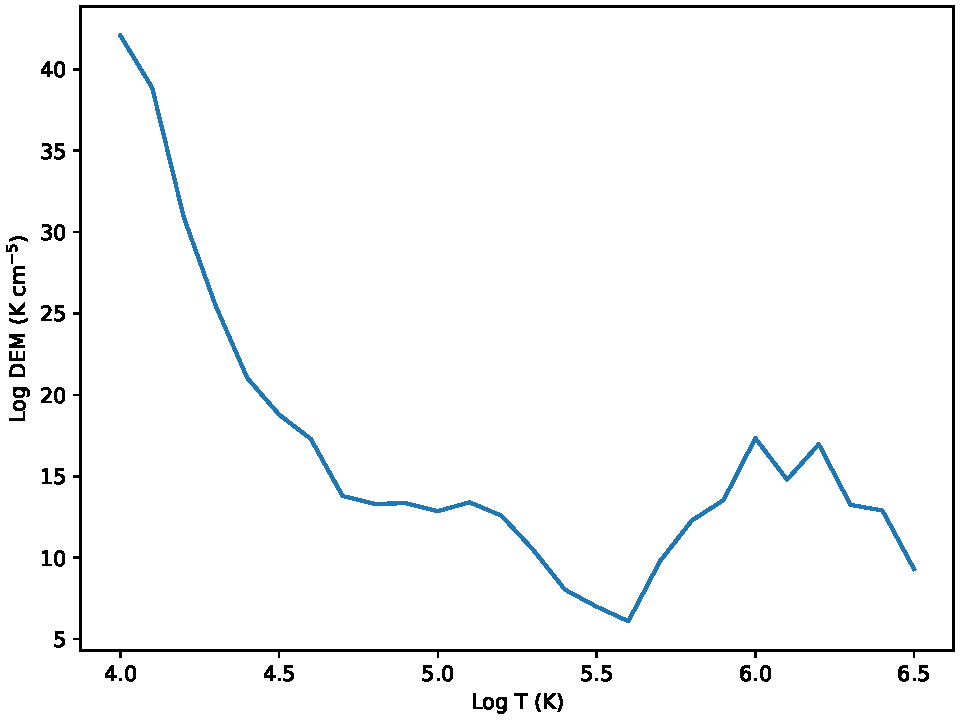
\includegraphics[width=\linewidth]{fit_dem}
		\caption{Best fit DEM used to generate the final synthetic MOSES images.}
		\label{fig:dem}
	\end{figure}

	\begin{figure}
		\centering
		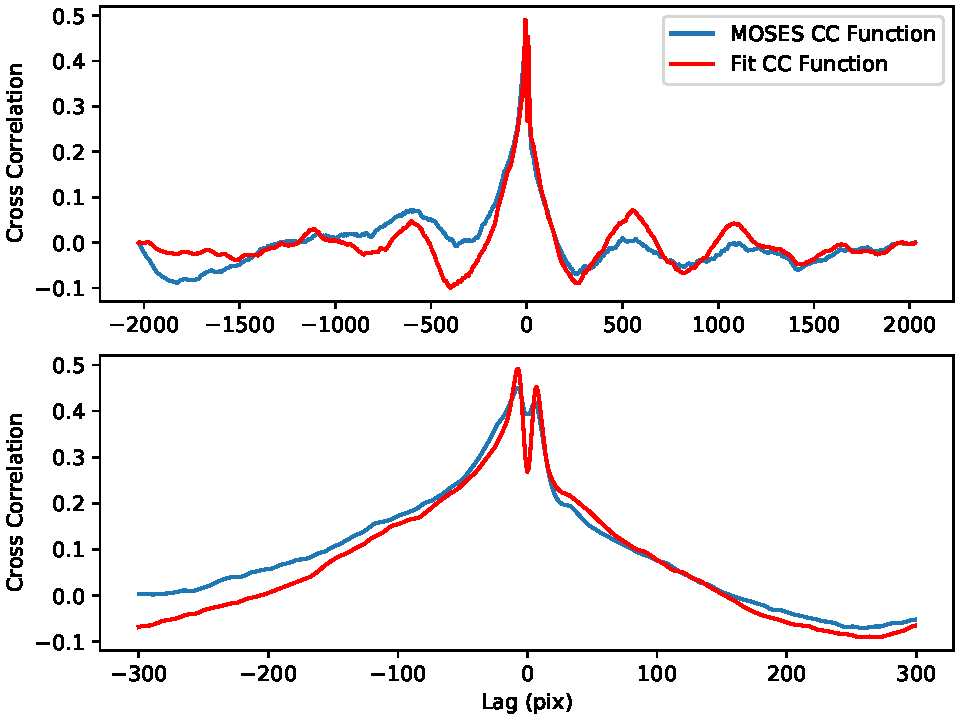
\includegraphics[width=\linewidth]{fit_cc}
		\caption{The top panel shows the entire mean cross-correlation along image rows of of the MOSES (blue) and synthetic (red) difference images.  The bottom panel shows a zoomed in view of the same function in order to highlight features near zero lag.}
		\label{fig:fit_cc}
	\end{figure}
	
	We find good agreement between our synthetic data of best fit and the MOSES data.
	Figure \ref{fig:fit_cc} compares the mean cross-correlation of the difference image rows from the slightly blurred MOSES data, to same cross-correlation of the synthetic data.
	Comparing the two curves shows notable agreement in a few places including around zero lag and all positive lags.
	Negative lags match less closely, although the shape between zero and approximately -600 pixels is similar. 
	Considering that we have attempted to use a single DEM to represent the quiet Sun over a very large field of view, we think the agreement is remarkable.

	
	\begin{figure}
		\centering
		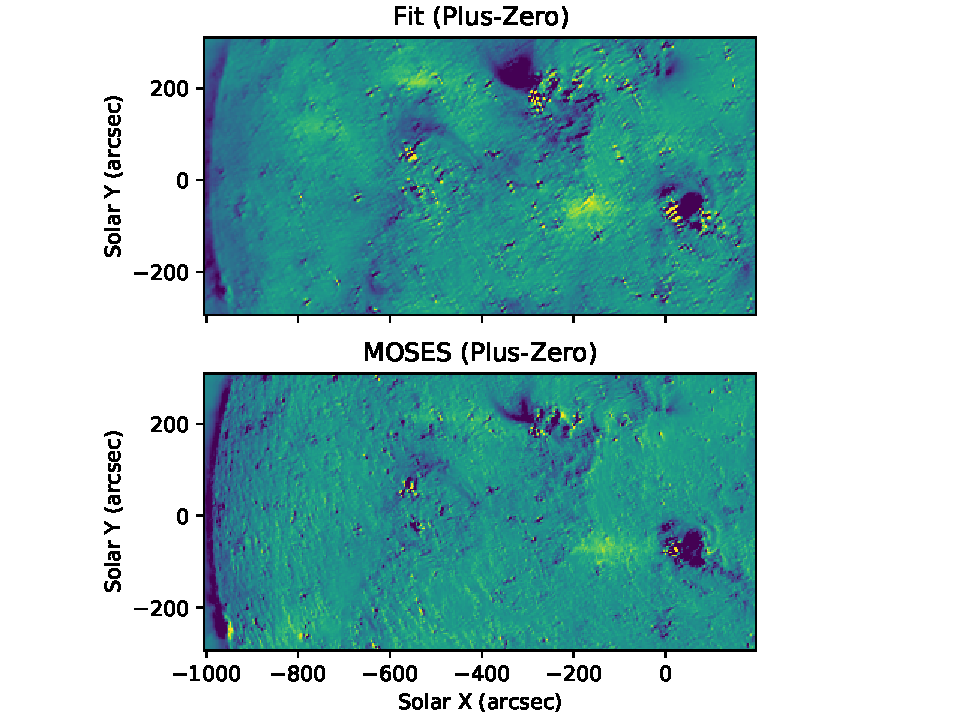
\includegraphics[]{fit_dif_images}
		\caption{The $I_{+1}-I_0$ difference image, also shown in Figure \ref{fig:moses_super}c, along side the same difference image prepared from the synthetic MOSES images of best fit.  Identical regions 1-3 are boxed in each image for comparison.}
		\label{fig:dif_image_fit}
		
	\end{figure}
	
	A synthetic difference image of best fit ($I'_{+1}$ minus $I'_0$) is shown along with the corresponding MOSES difference image in Figure \ref{fig:dif_image_fit}.
	In the synthetic difference image each feature identified in Figure \ref{fig:moses_super} has been successfully reproduced.
	The dark imprint of the ``wishbone'' (region 1) and nearby active region (region 2), are clearly visible and are adjacent to lighter smears of intensity to their left.
	Region 3, while not as sharp in the synthetic images, is reproduced at the limb with the same close separation between the positive and negative lobes.
	
	\begin{figure}
		\centering
		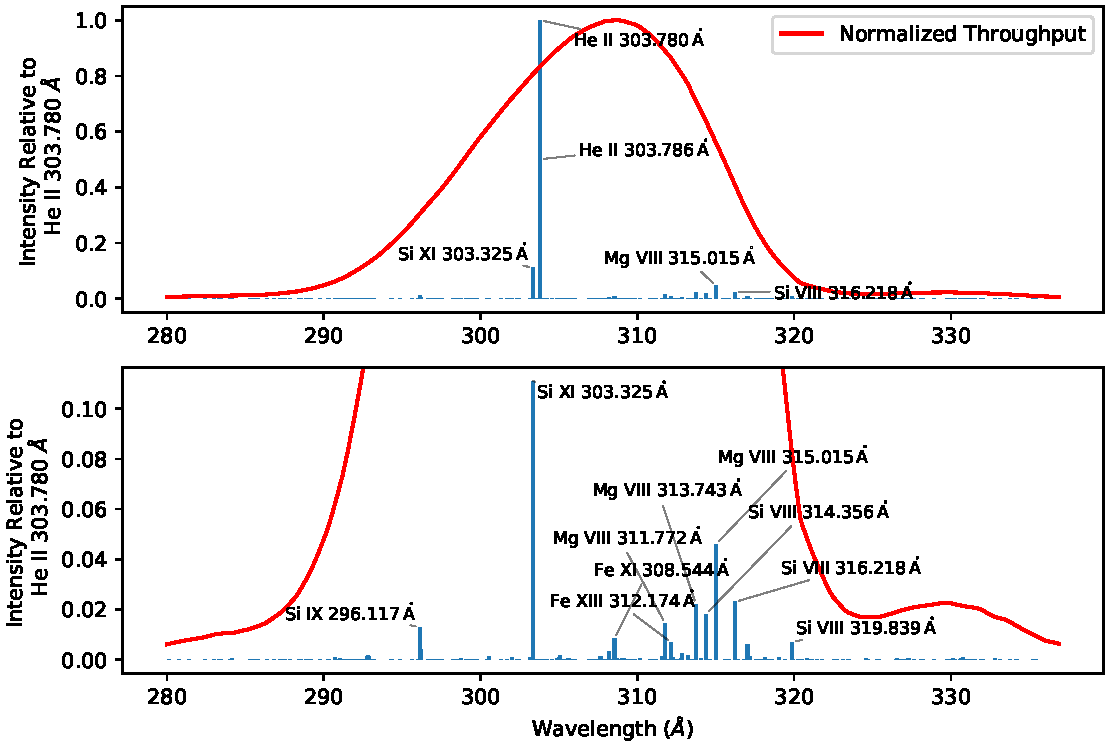
\includegraphics[width=\linewidth]{fit_spectrum}
		\caption{Using the DEM of best fit shown in Figure \ref{fig:dem} we generated the above synthetic spectrum using Chianti. Each line intensity has also been weighted by the wavelength dependent throughput of the MOSES optical system (normalized and shown in red).}
		\label{fig:spectrum}
	\end{figure}
	\begin{table}
		\begin{center}
			\caption{Average MOSES Image Spectral Content}
			\label{table:spectral_content}
			\begin{tabular}{l|r}
				\hline
				Ion & Contribution \\
				\hline
				He\,\textsc{ii} & 80.55\% \\
				Si\,\textsc{xi} & 8.37\% \\
				Mg\,\textsc{viii} & 4.14\% \\
				Si\,\textsc{viii} & 2.65\% \\
				Si\,\textsc{ix} & 1.33\% \\
				Fe\,\textsc{xiii} & 1.29\% \\
				Other & 1.67\% \\ 
				\hline
			\end{tabular}
		\end{center}
	\end{table} 
	
	
	Using the DEM of best fit we also generated an average spectrum for the MOSES data weighted by instrument's the wavelength dependent throughput (Figure \ref{fig:spectrum}).
	The synthetic spectrum of best fit was generated using the same constant pressure, abundance file, and spectral range as was used in the forward model (Section \ref{sec:fomod}).
	MOSES images are dominated by the He\,\textsc{ii} doublet near 303.7\,\AA.
	\sixi, while much dimmer than He\,\textsc{ii}, has the second highest intensity and represents approximately 8 percent of the total intensity.
	The other notable, and unexpected contribution to the image intensity is from the host of lines between 310 and 320 angstroms, the brightest being from Mg\,\textsc{viii} and Si\,\textsc{viii}.
	Table \ref{table:spectral_content} shows the total intensity contribution from each of the brightest ions.  
	

	
\section{Discussion and Conclusions}\label{sec:conclusion}

	MOSES was successful in its goal of capturing solar images in the \heii \ emission line.
	Despite the use of a narrowband multi-layer coating on both the primary and secondary optics, MOSES captured several solar features not easily attributed to the dominant \heii \ or nearby strong \sixi \ lines.
	In order to identify and quantify the spectral content of these additional features we cross-correlated two MOSES difference images and identified peaks in correlation as significant and indicative of spectral contamination.
	Using a forward model that combines four co-temporal EIT images with synthetic spectra from Chianti we created synthetic MOSES difference images with known spectral content that could be cross-correlated and compared to the MOSES difference image cross-correlation function.
	By varying the DEM used we modified the spectral content of the synthetic MOSES data until we minimized the differences between the synthetic and real cross-correlation functions, the results of which are displayed in Section \ref{sec:results}.
	
	Compared to other solar DEMs, like those included in the Chianti software package, our DEM of best fit (Figure \ref{fig:dem}) shows a huge increase in emission measure between log T = 4-5\,K.
	This result is artificial and is caused by a significant lack of modeled intensity in the \heii \ emission line when using Chianti.
    The \heii\ intensity is low by up to an order of magnitude when modeled under classical assumptions, and its lack of emission  has been attributed to a host of factors including a lack of ionization equilibrium \citep{Golding2017}.
	Since the MOSES passband is absent of any other bright, cool lines ($<$.1\,MK) our fit can increase the emission measure at low temperatures resulting in an increase in the intensity of \heii \ alone, allowing for a more accurate intensity ratio between it and nearby hot emission lines like \sixi.
	We find an average line ratio between \heii\ and \sixi\ intensities of $\approx$ 10:1 which is comparable to ratios measured by other slit spectrographs in regions of moderate solar activity \citep{Cushman1978}.
	
	It is also important to note that although we chose to use a DEM as the basis of our fit, we do not consider it to be an accurate average DEM of the sun across the MOSES field of view.
	The formation temperatures of lines within the MOSES passband very sparsely cover the range of log T = 4 - 6.5, allowing multiple DEMs to represent the same spectral content.
	Despite the parameter space being very degenerate, we chose to vary emission measure rather than individual line intensities to ensure our final fits have physically realizable line ratios.
	
	The temperature coverage of EIT, used to create the synthetic data, is also very sparse.
	Luckily, the dominant line in each of the four included EIT images have peak formation temperatures that closely match the peak formation temperatures of the brightest lines imaged by MOSES.  
	The four EIT channels used, He\,\textsc{ii}\,304\,\AA, Fe\,\textsc{ix}\,171\,\AA,  Fe\,\textsc{xii}\,195\,\AA, Fe\,\textsc{xv}\,284\,\AA, have peak formation temperature of log T = 4.7\,K, 5.9\,K, 6.2\,K and 6.3\,K respectively, calculated using Chianti.  
	The bright, hotter lines imaged by MOSES, namely from Mg\,\textsc{viii}, Si\,\textsc{viii}, and Si\,\textsc{xi}, have peak formation temperatures of log T = 5.9\,K, 5.95\,K, and 6.2\,K respectively. 
	This allows for synthetic MOSES data with key intensity contributors well represented, as is evident when comparing features in the synthetic difference images of best fit to those in the MOSES difference images (Figure \ref{fig:dif_image_fit}).
	
	The most mysterious features in the MOSES difference images, those that motivated this study, are regions 1 (the ``wishbone'') and 2 identified in Figures \ref{fig:moses_super} and \ref{fig:dif_image_fit}.
	These two features are very coronal in appearance and easily identifiable in the hotter EIT channels, but they cannot be attributed to the most obvious source of contamination in any He\,\textsc{ii} image, \sixi, due to the lack of positive component $\approx$\sixipix\ pixels away like that seen in region 3.
	The presence of a faint, light smear left of the wishbone indicates that it is from emission at longer wavelengths than \heii, but a lack of clear positive wishbone makes it difficult to attribute it to a single contaminant line.
	The best fit spectrum (Figure \ref{fig:spectrum}) shows a host of lines between 310 and 320 angstroms, mostly emitted by the Mg\,\textsc{viii} and Si\,\textsc{viii} ions, the strongest being \spectralline{Mg}{viii}{315}\ (Also identified by \citet{Rust2017}).
	Despite their individually weak intensity, combined they contribute on order the same intensity as \sixi.
	Due to spectral dispersion, these lines are very faint in the MOSES outboard order and could likely be neglected.
	In the zero order image, all of these faint lines land in the same place on the detector which is why these features appear so clearly when subtracting the zero order.	
	The intensity contribution from lines other than \heii\ and \sixi\ amounts to around ten percent of the total intensity in the zero order and comes from tens of lines that may be easily overlooked during analysis or instrument development.
	Some of these lines are shifted hundreds of pixels, causing feature within the field of view of the MOSES zero order to be shifted out and those outside to be shifted in the outboard orders.
	This results in different total intensities existing in each spectral order, which could lead to confusion when comparing orders during inversion.
	
	While overlapping intensity from different spectral lines is inevitable in this type of instrument, the use of a zero order (undispersed) image and a lack of clearly defined field of view in MOSES exacerbates the problem of spectral contamination.
	ESIS \citep{ESIS,Parker2021}, our second-generation rocket borne slitless spectrograph, builds off the MOSES concept and improves on it in several ways. 
	The most relevant improvements include an intermediate focal plane and field stop, that clearly defines the instrument field of view, and four channels rather than three, none of which is undispersed.
	Including a field stop defines the same field of view for every channel and solves the problem of highly shifted features existing in some orders, but not others.
	Even with a clearly defined field of view features in the zero order image would still have intensity from lines that are dispersed off the detector in the outboard orders.
	The ambiguity of spectral content makes it difficult to compare its intensity to outboard orders without DEM forward modeling. 
	Using all dispersed orders, as is done in ESIS, makes it much easier to compare the intensity of solar features from specific emission lines, and tends to reduce the effect of contaminant lines on measured intensity by dispersing them across the image. 
	We think this approach will prove particularly advantageous with a high dispersion instrument whose chief science objective is to resolve the profiles of strong lines. 
	The considerations are rather different when the instrument is designed from the start to reconstruct DEMs, as with COSIE \citep{winebarger2019}.	
	
	In the MOSES design, the zero order was intended to improve the spatial resolution, which is otherwise blurred by the line profiles in the horizontal direction. 
	It served very effectively in this role. 
	With ESIS, we oriented the dispersion of its four channels in four different directions. 
	Each ESIS channel has its highest resolution in the direction perpendicular to the dispersion, and together they are able to separate closely spaced features with any orientation. 
	As our inversion skill improves, we will learn whether this approach to high resolution imaging is  as successful as the zero order.
	
	In summary, we have developed a forward model of the MOSES instrument that combines the Chianti database and images from EIT to form synthetic MOSES data with known spectral content.
	Our fits match the MOSES data well and indicate that the unexpected solar features identified in MOSES difference images are composed of tens of dim lines that, in the aggregate, contribute approximately 10 percent of the average intensity in the zero order image and are smeared over many hundreds of pixels in the outboard orders.
	This unexpected spectral content makes it difficult to compare the intensity of certain features between spectral orders and, if not properly accounted for, could lead to poor convergence when inverting slitless spectrograph data.
	Our analysis led us to comment on the advantages and disadvantages of zero order imaging in a slitless spectrograph. These considerations should aid in the design of future instruments of this type.
	
	
	
	
	
	
